\begin{frame}{Variance reduction: MLMC}
  \begin{figure}
    \centering
    \includegraphics[scale=0.43]{src/imgs/mesh_mlmc}
  \end{figure}
\end{frame}

\begin{frame}[noframenumbering]{Variance reduction: Further potential}
  \begin{figure}
    \centering
    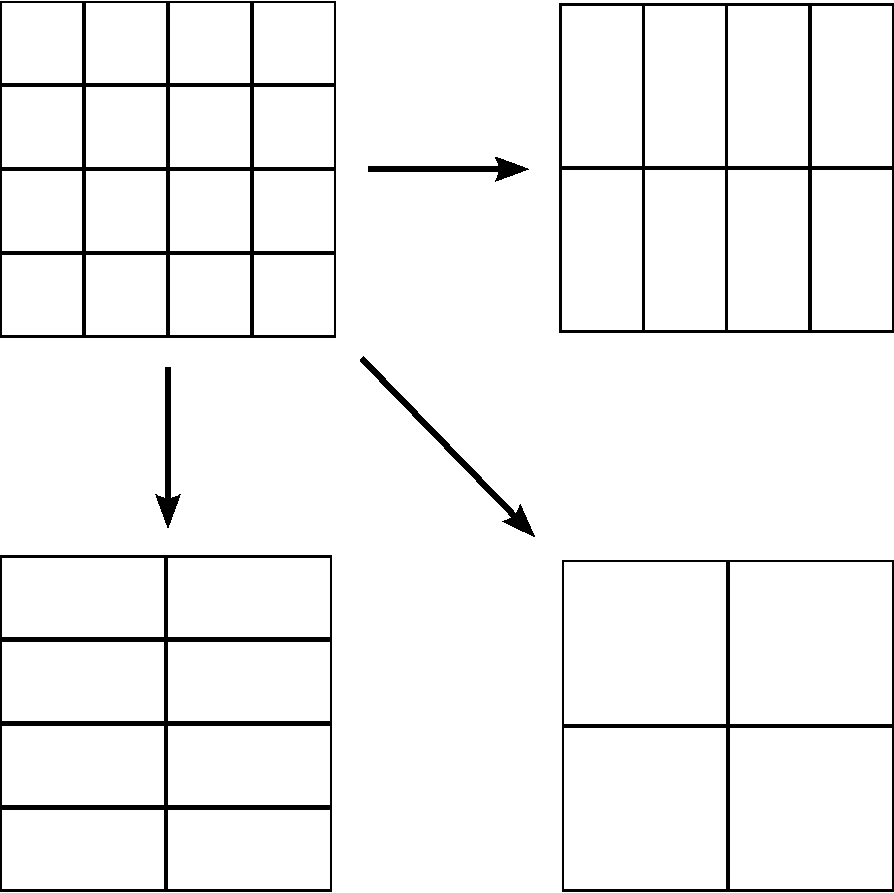
\includegraphics[scale=0.43]{src/imgs/mesh_mimc}
  \end{figure}
\end{frame}

%%%%%%%%%%%%%%%%%%%%%%%%%%%%%%%%%%%%%%%%%%%%%%%%%%%%%%%%%%
\subsection{Multi-Index Monte Carlo (MIMC)}
%%%%%%%%%%%%%%%%%%%%%%%%%%%%%%%%%%%%%%%%%%%%%%%%%%%%%%%%%%
\begin{frame}{MIMC Estimator}
Consider discretization parameters possibly different in each direction
\[
   {h_{i,\alpha_i} = h_{i,0}\, \beta_i^{-\red{\alpha_i}}}
\]
with $\beta_i > 1$. For a multi-index $\red{\valpha} = \left( \red{\alpha_i} \right)_{i=1}^d \in \nset^d$, we denote by $\blue{g}_{\red{\valpha}}$ the approximation  of $\blue{g}$ calculated using a discretization defined by
$\red{\valpha}$.

\onslide<2->
\medskip
For $i=1,\ldots,d,$ define the first order  difference operators
  \begin{align*}
    \blue{\Delta_i}  g_\valpha = \begin{cases}
       g_\valpha & \text{if } \alpha_i=0, \\
       g_{\valpha} -  g_{\valpha-\blue{\vec e_i}} & \text{if } \alpha_i > 0,
      \end{cases}
    \end{align*}
  \end{frame}
  \begin{frame}{MIMC Estimator}
    Construct the first order mixed difference
    \[
      \blue{\Delta}  g_\valpha =\blue{\left( \otimes_{i=1}^d  \Delta_i\right)}
      g_\valpha {=\red{\sum_{\mathbf{j}\in\{0,1\}^d} (-1)^{|\mathbf{j}|}} g_{\valpha-\red{\mathbf{j}}}}
    \]
    with $|\mathbf{j}| = \sum_{i=1}^d j_i$. Requires $2^d$ evaluations
    of $g$ on different grids.
\end{frame}

\begin{frame}\frametitle{Example: Computing $g_\valpha$ in $d=2$}
%\begin{example*}[$d=2$]
    \begin{minipage}[b]{0.6\linewidth}
For $\valpha = (\alpha_1,\alpha_2)$, we have
  \begin{align*}
    \Delta g_{(\alpha_1,\alpha_2)} &= \Delta_2 (\Delta_1 g_{(\alpha_1,\alpha_2)})\\
    &= \Delta_2 \left( g_{\alpha_1,\alpha_2} - g_{\alpha_1-1,\alpha_2} \right) \\
    &=  \blue{g_{\alpha_1,\alpha_2}} - \blue{g_{\alpha_1\red{-1},\alpha_2}} \\
    &\quad - \blue{g_{\alpha_1,\alpha_2\red{-1}}} + \blue{g_{\alpha_1\red{-1},\alpha_2\red{-1}}}.
  \end{align*}

\vspace{1.5cm}
\phantom{a}
\end{minipage}
\hspace{0.375cm}
\begin{minipage}[b]{0.3\linewidth}
\begin{center}
    \def\svgwidth{3cm} %% Creator: Inkscape inkscape 0.48.4, www.inkscape.org
%% PDF/EPS/PS + LaTeX output extension by Johan Engelen, 2010
%% Accompanies image file 'temp.pdf' (pdf, eps, ps)
%%
%% To include the image in your LaTeX document, write
%%   \input{<filename>.pdf_tex}
%%  instead of
%%   \includegraphics{<filename>.pdf}
%% To scale the image, write
%%   \def\svgwidth{<desired width>}
%%   \input{<filename>.pdf_tex}
%%  instead of
%%   \includegraphics[width=<desired width>]{<filename>.pdf}
%%
%% Images with a different path to the parent latex file can
%% be accessed with the `import' package (which may need to be
%% installed) using
%%   \usepackage{import}
%% in the preamble, and then including the image with
%%   \import{<path to file>}{<filename>.pdf_tex}
%% Alternatively, one can specify
%%   \graphicspath{{<path to file>/}}
%%
%% For more information, please see info/svg-inkscape on CTAN:
%%   http://tug.ctan.org/tex-archive/info/svg-inkscape
%%
\begingroup%
  \makeatletter%
  \providecommand\color[2][]{%
    \errmessage{(Inkscape) Color is used for the text in Inkscape, but the package 'color.sty' is not loaded}%
    \renewcommand\color[2][]{}%
  }%
  \providecommand\transparent[1]{%
    \errmessage{(Inkscape) Transparency is used (non-zero) for the text in Inkscape, but the package 'transparent.sty' is not loaded}%
    \renewcommand\transparent[1]{}%
  }%
  \providecommand\rotatebox[2]{#2}%
  \ifx\svgwidth\undefined%
    \setlength{\unitlength}{173.00908456bp}%
    \ifx\svgscale\undefined%
      \relax%
    \else%
      \setlength{\unitlength}{\unitlength * \real{\svgscale}}%
    \fi%
  \else%
    \setlength{\unitlength}{\svgwidth}%
  \fi%
  \global\let\svgwidth\undefined%
  \global\let\svgscale\undefined%
  \makeatother%
  \begin{picture}(1,0.93172362)%
    \put(0,0){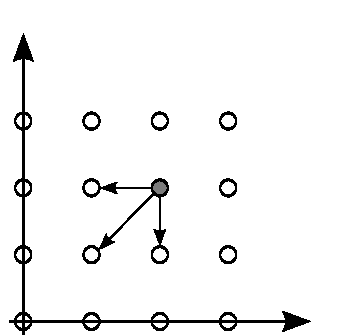
\includegraphics[width=\unitlength]{delta.pdf}}%
    \put(-0.00714377,0.85933761){\color[rgb]{0,0,0}\makebox(0,0)[lb]{\smash{$\alpha_1$}}}%
    \put(0.86940741,0.02589459){\color[rgb]{0,0,0}\makebox(0,0)[lb]{\smash{$\alpha_2$}}}%
  \end{picture}%
\endgroup%

\vskip 0.2cm
  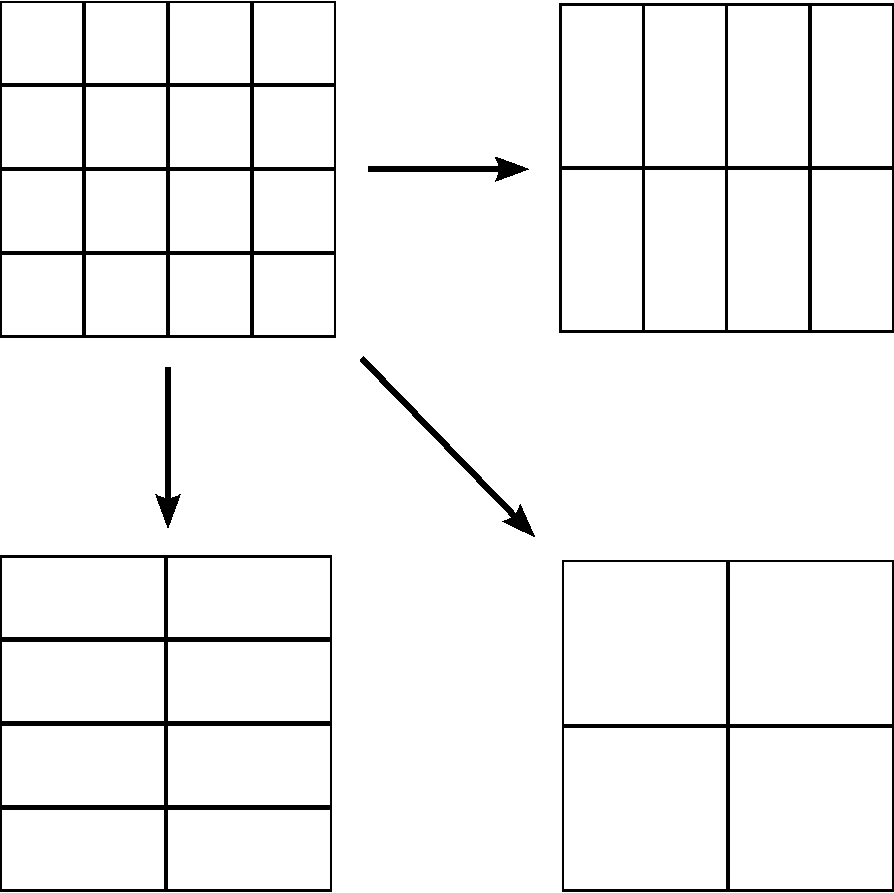
\includegraphics[scale=0.25]{src/imgs/mesh_mimc}
  \end{center}
\end{minipage}
\end{frame}

\begin{frame}\frametitle{MIMC Estimator}
Then, assuming that
\[
  \E{g_\valpha}\rightarrow\E{g} \quad \text{ as } \quad \alpha_i\rightarrow \infty \;\; \text{for all $i=1,\ldots,d$,}
\]
it is not difficult to see that
\[
  \E{g}= \sum_{\valpha\in\nset^d} \E{\blue{\Delta}g_\valpha} \uncover<2->{\approx \sum_{\valpha\in\red{\mathcal I}} \E{\blue{\Delta}g_\valpha}}
\]
\onslide<2->
where $\red{\mathcal I} \subset \nset^d$  is a \emph{properly chosen} index set.


\onslide<3->
\medskip
As in MLMC, appoximating each term by independent MC samplers,
the MIMC estimator can be written as
  \begin{align*}
    \mathcal A_{\text{MIMC}}[g ; \red{\mathcal
    I}] = \sum_{\valpha \in \red{\mathcal
    I}}\frac{1}{M_\valpha}
    \sum_{m=1}^{M_\alpha}  \blue{\Delta} g_\valpha(\omega_{\valpha,m})
  \end{align*}
with \emph{properly chosen} sample sizes $(M_\valpha)_{\valpha\in\red{\mathcal I} }$.
\end{frame}

% \begin{frame}
% Our objective is to build an estimator $\mathcal{A}=   \mathcal A_{\text{MIMC}} $  where
% \begin{equation}\label{eq:accuracy_constr}
% %\prob{
%  P(
%  |\mathcal{A} - \E{g}| \leq \tol
%  )\
%  %}\
%  \ge 1-\epsilon
% \end{equation}
% %
% for a given accuracy  $\tol$ and a given confidence level determined by $0<\epsilon \ll 1$.
% We instead impose the following, more restrictive, two constraints:
% \begin{align}
%   \label{eq:bias_const} \text{\bf Bias constraint:}  & &\blue{|\E{\mathcal{A}-S}|} \leq \blue{(1-\theta)} \tol, \\
%   \label{eq:stat_const0} \text{\bf Statistical constraint:}& & P\left( \red{|\mathcal{A} - \E{\mathcal{A}}|} \leq \red{\theta}\tol \right)
%  \ge 1-\epsilon.
%  \end{align}

%  For a given fixed $\theta \in (0,1)$.
%  Moreover, motivated by the asymptotic normality of the estimator,
%  $\mathcal{A}$, we approximate \eqref{eq:stat_const0} by
% \begin{equation}\label{eq:stat_const}
% \var{\mathcal{A}} \leq \left( \frac{\theta \tol}{C_\epsilon} \right)^2.
%  \end{equation}
% % Moreover, $1-\epsilon$ is the confidence level corresponding to the constraint \eqref{eq:stat_const}
% Here, $0<C_\epsilon$ is such that $\Phi(C_\epsilon) = 1 - \frac{\epsilon}{2}$, where $\Phi$ is the cumulative distribution function of a standard normal random variable.
% \end{frame}


\begin{frame}{Assumptions for MIMC}
For every $\valpha$, we assume the following
\begin{align*}
  &\textbf{Assumption 1 (Bias)}: &E_\valpha =\left|\E{\Delta
      g_\valpha}\right| &\propto \prod\nolimits_{i=1}^{\red{d}}
  \beta_i^{-\alpha_i w_i}\\
  &\textbf{Assumption 2 (Variance)}:& V_\valpha =\var{\Delta
    g_\valpha} &\propto \prod\nolimits_{i=1}^{\red{d}} \beta_i^{-\alpha_i s_i},\\
  &\textbf{Assumption 3 (Work)}: &W_\valpha = \text{Work}( \Delta
  g_\valpha) &\propto \prod\nolimits_{i=1}^{\red{d}}
  \beta_{i}^{\alpha_i \gamma_i} ,
\end{align*}
For positive constants $\gamma_i, w_i, s_i < 2w_i$ and for $i = 1
\ldots d$.

    \begin{align*}
      \text{Work}({\text{MIMC}}) =& \sum_{\valpha \in \mathcal I}
      {M_\valpha} W_{\valpha} \propto \sum_{\valpha\in\mathcal I}
      {M_\valpha} \, \left( \prod\nolimits_{i=1}^{\red{d}} \beta_{i}^{\alpha_i
          \gamma_i} \right).
    \end{align*}

\end{frame}

\begin{frame}\frametitle{Remark on product rates}

\begin{itemize}
\item The {\bf Assumptions 1 \& 2} in MIMC that the rates for each $\valpha$ are \emph{products of 1D rates}
\[
  E_\valpha \propto \prod\nolimits_{i=1}^{\red{d}}
  \beta_i^{-\alpha_i w_i}, \qquad V_\valpha \propto \prod\nolimits_{i=1}^{\red{d}} \beta_i^{-\alpha_i s_i}
\]
are stronger than the corresponding assumptions in MLMC.

\item<2-> They imply existence of \blue{mixed derivatives} of the solution
  of the PDE (and possibly the solution of the adjoint problem
  associated to the functional $\Psi$), as opposed to standard
  derivatives for MLMC.
\end{itemize}

\end{frame}

\begin{frame}{Optimal index set}
  \begin{minipage}[m]{0.7\linewidth}
    \begin{center}
      \def\svgwidth{7cm} s%% Creator: Inkscape inkscape 0.48.4, www.inkscape.org
%% PDF/EPS/PS + LaTeX output extension by Johan Engelen, 2010
%% Accompanies image file 'total_degree.pdf' (pdf, eps, ps)
%%
%% To include the image in your LaTeX document, write
%%   \input{<filename>.pdf_tex}
%%  instead of
%%   \includegraphics{<filename>.pdf}
%% To scale the image, write
%%   \def\svgwidth{<desired width>}
%%   \input{<filename>.pdf_tex}
%%  instead of
%%   \includegraphics[width=<desired width>]{<filename>.pdf}
%%
%% Images with a different path to the parent latex file can
%% be accessed with the `import' package (which may need to be
%% installed) using
%%   \usepackage{import}
%% in the preamble, and then including the image with
%%   \import{<path to file>}{<filename>.pdf_tex}
%% Alternatively, one can specify
%%   \graphicspath{{<path to file>/}}
%%
%% For more information, please see info/svg-inkscape on CTAN:
%%   http://tug.ctan.org/tex-archive/info/svg-inkscape
%%
\begingroup%
  \makeatletter%
  \providecommand\color[2][]{%
    \errmessage{(Inkscape) Color is used for the text in Inkscape, but the package 'color.sty' is not loaded}%
    \renewcommand\color[2][]{}%
  }%
  \providecommand\transparent[1]{%
    \errmessage{(Inkscape) Transparency is used (non-zero) for the text in Inkscape, but the package 'transparent.sty' is not loaded}%
    \renewcommand\transparent[1]{}%
  }%
  \providecommand\rotatebox[2]{#2}%
  \ifx\svgwidth\undefined%
    \setlength{\unitlength}{279.65738473bp}%
    \ifx\svgscale\undefined%
      \relax%
    \else%
      \setlength{\unitlength}{\unitlength * \real{\svgscale}}%
    \fi%
  \else%
    \setlength{\unitlength}{\svgwidth}%
  \fi%
  \global\let\svgwidth\undefined%
  \global\let\svgscale\undefined%
  \makeatother%
  \begin{picture}(1,0.94890322)%
    \put(0,0){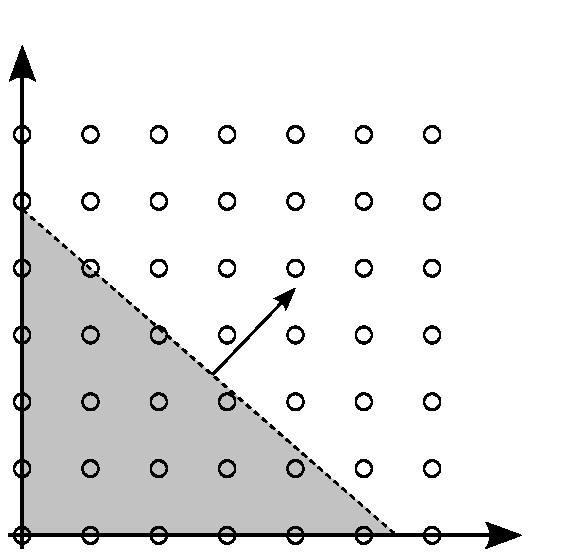
\includegraphics[width=\unitlength]{total_degree.pdf}}%
    \put(0.43355946,0.44597791){\color[rgb]{0,0,0}\makebox(0,0)[lb]{\smash{$L$}}}%
    \put(-0.00441947,0.90412186){\color[rgb]{0,0,0}\makebox(0,0)[lb]{\smash{$\alpha_1$}}}%
    \put(0.91920934,0.0160196){\color[rgb]{0,0,0}\makebox(0,0)[lb]{\smash{$\alpha_2$}}}%
  \end{picture}%
\endgroup%

    \end{center}
  \end{minipage}
  \hspace{0.375cm}
  \begin{minipage}[m]{0.2\linewidth}
    Or find it adaptively!
  \end{minipage}
\end{frame}

\begin{frame}{Fully Isotropic Case: Rough noise case}
 % \fontsize{10pt}{7.2}\selectfont
  Assume  $w_i = w$, $s_i = s < 2w$, $\beta_i = \beta$ and $\gamma_i =
  \gamma$ for all $i \in \indset$. Then the optimal work is
  \begin{align*}
    \text{Work}({\text{MC}})  &= \Order{\tol^{-2 - \blue{\frac{\red{d}\gamma}{w}}}}. \\
    \text{Work}({\text{MLMC}}) &= \begin{cases}
  \Order{\tol^{-2}}, & s > \red{d}\gamma, \\
  \Order{\tol^{-2} \left(\log\left(\tol^{-1}\right)\right)^2}, \hskip 4em & s = \red{d}\gamma, \\
  \Order{\tol^{-\left(2 +\blue{\frac{(\red{d}\gamma-s)}{w}}\right)}},  & s < \red{d}\gamma. \\
\end{cases} \\
%     \text{Work(MIMC, FT)} &= \begin{cases}
%   \Order{\tol^{-2}}, & s > \gamma, \\
%   \Order{\tol^{-2} \left(\log(\tol^{-1})\right)^{2\red{d}}}, \hskip 4em & s = \gamma, \\
%   \Order{\tol^{-\left(2 + \frac{\red{d}(\gamma-s)}{w}\right) }},  & s < \gamma,
% \end{cases}\\
    \text{Work}({\text{MIMC}}) &= \begin{cases}
  \Order{\tol^{-2}}, & s > \gamma, \\
  \Order{\tol^{-2} \left(\log\left(\tol^{-1}\right)\right)^{2\red{d}}}, & s = \gamma, \\
  \Order{\tol^{-\left(2 + \blue{\frac{\gamma-s}{w}}\right) } \log\left(\tol^{-1}\right)^{(\red{d}-1)\frac{\gamma-s}{w}}},  & s < \gamma.
  \end{cases}
\end{align*}
\end{frame}


%%% Local Variables:
%%% mode: latex
%%% TeX-master: "../main"
%%% End:
